\documentclass[a4paper,11pt,onecolumn]{article}
\usepackage[latin1]{inputenc}
\usepackage[english]{babel}
\usepackage{amsmath}
\usepackage{amsfonts}
\usepackage{amssymb}
\usepackage{cuted}

\usepackage{titling}
\usepackage{nomencl}
\usepackage{geometry}
\geometry{%
letterpaper, % a4paper
left=   1.5 cm,
right=  1.5 cm,
top=    1.5 cm,
bottom= 1.5 cm,
}\usepackage{siunitx}
\usepackage[style=ieee,backend=bibtex]{biblatex}
\usepackage[font={small}]{caption}
\usepackage{graphicx}
\usepackage{color}

\usepackage{booktabs}
\usepackage{threeparttable}
\usepackage{fancyhdr}
\usepackage{float}
\usepackage{multirow}
\usepackage{wrapfig}
\usepackage{caption}
\usepackage{subcaption}
\usepackage{varioref}
\usepackage{textcomp}
\usepackage{xspace}
\usepackage[activate={true,nocompatibility},final,tracking=true,kerning=true
,spacing=nonfrench,factor=1100,stretch=10,shrink=10]{microtype}

% Reduce tracking around small caps to 40%
\SetTracking{encoding={*}, shape=sc}{40}

% Document info.
\author{George Arthur Hall}
\title{CFD Analysis Using Solidworks\textregistered}
\date{\today}

% Header and footer.
\pagestyle{fancy}
\fancyhf{}
\lhead{\thetitle}
\rhead{\theauthor}
\cfoot{\thepage}
\renewcommand{\headrulewidth}{0pt}
\renewcommand{\footrulewidth}{0pt}

%%%%%%%%%%%%%%%%
% BEGIN DOCUMENT
%%%%%%%%%%%%%%%%
\begin{document}
%%%%%%%%%%%%%%%%
% THEORY
%%%%%%%%%%%%%%%%
\section{Theory}

Computational Fluid Dynamics (CFD) is a powerful tool that allows
flow problems
which do not have a known analytical solution to be solved [1]. It is
used to provide fast testing of new design concepts, gather detailed
information of process conditions even for where measurements are difficult and
to further our understanding of process performance [2]. However, CFD is
a dangerous tool because if used without a full understanding of the physical
process which is occurring, large errors can easily amount, which is why the
results of simulations are often compared with rough theoretical solutions to
validate whether they are correct or not. 


When using Solidworks\textregistered~the following steps must
be performed by the user when carrying out CFD computation:
\begin{itemize}
\renewcommand\labelitemi{--}
\item Specify fluid and thermodynamic properties 
\item Define computational domain
\item Set mesh
\item Apply Boundary conditions
\item Specify goals
\end{itemize}


Within Solidworks\textregistered~flow analysis the following conservation laws
are solved:
\begin{itemize}
\renewcommand\labelitemi{--}
\item Conservation of momentum (Newton's $2^{nd}$ law)
\item Conservation of mass flow rate 
\item Conservation of energy 
\end{itemize}


For a simulation to be performed and the above stated conservation laws to be
solved, the simulation must be well poised; for this, knowledge of the fluids
viscosity~$\mu$, density $\rho$ and thermal conductivity $k$, are required.


When solving fluid flow problems, the area of interest - i.e. the area for
which we want our study to be performed - is defined by the computational
domain. This domain is then split into many small 'sub-domains' - i.e. a
mesh. Within each of these sub-domains the governing equations of the flow
problem
are discretised and solved. For fluid flow problems the finite volume numerical
method is employed [3] and solves the problem for each of the many sub-domains
within the mesh, these solutions are then combined and interpolation occurs to
provide a solution to the state of the fluid flow across the entire defined
computational domain.


Solidworks\textregistered~enables users to set properties of interest as
'goals', which then allows Solidworks\textregistered~to ensure that the value
of
that property is of a suitable nature before the simulation is to be considered
converged. Solidworks\textregistered~also allows for users to manually monitor
their simulations in real time. This is particularly useful when the
simulations being performed are computationally taxing as it allows users to
abort a simulation before potentially waiting long time periods to see that the
goals have not progressed as expected and that the simulation is misbehaving. 
%%%%%%%%%%%
% SECTION I
%%%%%%%%%%%
\section{Model I - "Pipe Flow"}

% Q6
\begin{figure}[ht!]
\centering
    	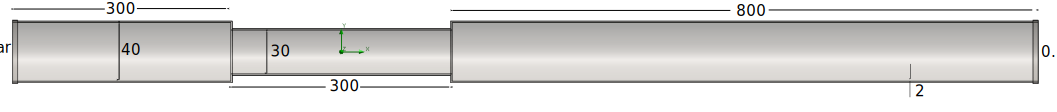
\includegraphics[width=0.75\textwidth]{q6.pdf}
    	\caption{Section view of fluid domain - all distance measurements in mm.}
\label{fig:q6}
\end{figure}
A 3D model was created within Solidworks\textregistered~ to simulate the flow
of water at 353~$k$ through a Steel pipe of surface roughness 0.045~$mm$, the
pipe having an inlet pressure of 1~bar and an outlet pressure of 0.6~bar , as
shown in Figure~\vref{fig:q6}.


After the fluid had passed through the restrictor section of the pipe it
undergoes an expansion, which leads to the occurrence of a recirculating region
within the pipe. To determine the percentage of the
outlet pipe which the recirculating region occupies, an Isosurface plot was
used to highlight the region of flow which had undergone a reversal in
sign (direction). The length of this recirculating region was then measured and
shown to be approximately 3.2~$\%$ of the outlet pipe.

% Q7
\begin{figure}
\centering
    	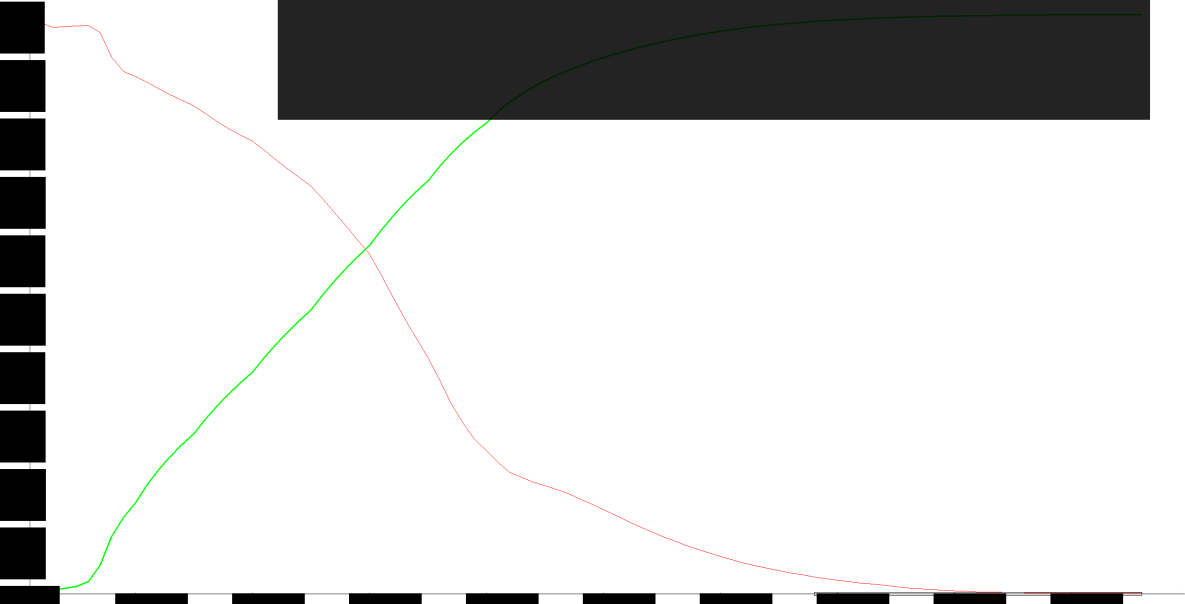
\includegraphics[height=5cm,width=0.5\textwidth]{q7.pdf}
    	\caption{Normalised goals plot for Average Static Pressure (Red), Average
Velocity(X) (Green)}
\label{fig:q13}
\end{figure}

% Q8 
\begin{figure}
\centering
    	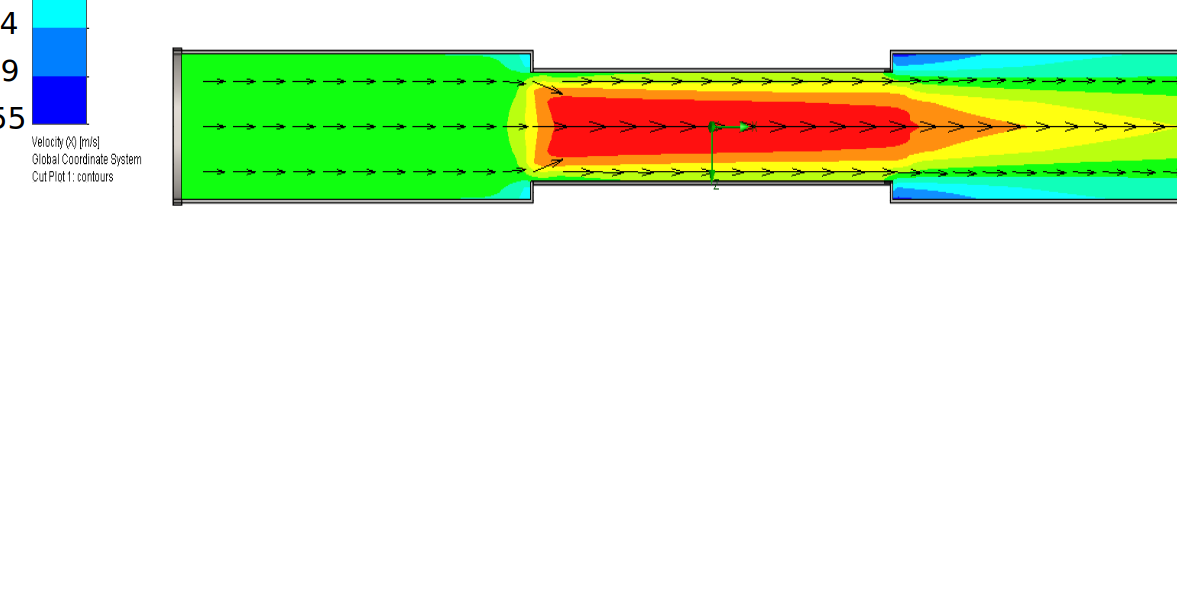
\includegraphics[width=0.75\textwidth]{q8.png}
    	\caption{Cut plot showing contours of magnitude of the fluid velocity and
vectors of fluid velocity}
\label{fig:q8}
\end{figure}

The average static pressure at the end of the restrictor section was then
determined by the placement of a 'lid' at the end of the restrictor section.
The
lid was then suppressed, simulation ran again and subsequently unsuppressed
so that the static pressure at that region could be read off as a surface
parameter on the lid - it was shown to be 41.9~kPa. To determine the mass
flow rate through the pipe the surface parameter was then employed for mass
flow
rate through this lid, and it was shown to be 26.3~$kgs^{-1}$.

As is good practise when performing CFD, this obtained value from the
simulation was to be verified through use of theoretical knowledge. Thus, the
pipe was split into three different sections and the following equation was
used
to
define the head loss,~$h$,

\begin{equation}
    \Delta h = \frac{\Delta P}{\rho g} = h_{Pipe1} + h_{Contraction1} +
h_{Pipe2} + h_{Expansion3} + h_{Pipe3}
\label{eq:h}
\end{equation}
This head loss is then used to calculate the mass flow rate, via the volumetric
flow rate. When using Equation \ref{eq:h} the flow is assumed to be fully
turbulent, thus the Moody diagram [6] is used to obtain the relevant
friction factors for this problem, and then this assumption that the flow is
fully turbulent is confirmed by calculating the Reynolds number, $Re$ from the
priorly obtained volumetric flow rate. The value of $Re$ was shown to be
1800000, which is substantially greater than the threshold value for turbulent
flow of 4000. Loss coefficients for $h_{Contraction1}$ and $h_{Expansion3}$
were found to be 0.125 and 0.191 respectively. The theoretical mass flow rate,
$\dot{m}$, was found to be 33.9~$kgs^{-1}$, which is similar to the value
obtained from the simulation and thus implies that the simulation is
trustworthy.


%%%%%%%%%%%%
% SECTION II
%%%%%%%%%%%%
\section{Model II - "Coolant Flow"}

% Q12
A further simulation was performed within Solidworks\textregistered~ this time
simulating the external flow of real Carbon dioxide ($CO_{2}$) at $453~K$
around a Uranium equilateral prism of sides $40~mm$ and depth $600~mm$ at a
temperature of $683~K$, as can be seen housed within a specified computational
domain in Figure 4. The $CO_{2}$ is at a pressure of 25~bar and a
velocity in the x-direction of $0.2~ms^{-1}$. For this simulation goals of
Average Static Pressure, Average velocity (X), Average Velocity (Y) and Average
Fluid Temperature were set, the calculation was set to run for 20~seconds
physical time and the progression of these goals across the time period can be
seen in Figure 5.

%Q12
\begin{figure}[ht!]
\centering
\label{fig:12}
\begin{subfigure}{.45\textwidth}
  \centering
  \includegraphics[width=\linewidth]{q12a.png}
  \caption{Isometric view of the computational domain}
\end{subfigure}
\begin{subfigure}{.45\textwidth}
  \centering
  \includegraphics[width=.7\linewidth]{q12ii.png}
  \caption{Computational domain dimension}
\end{subfigure}
\caption{Uranium Equilateral prism.}
\end{figure}

% Q13
\begin{figure}[ht!]
\centering
    	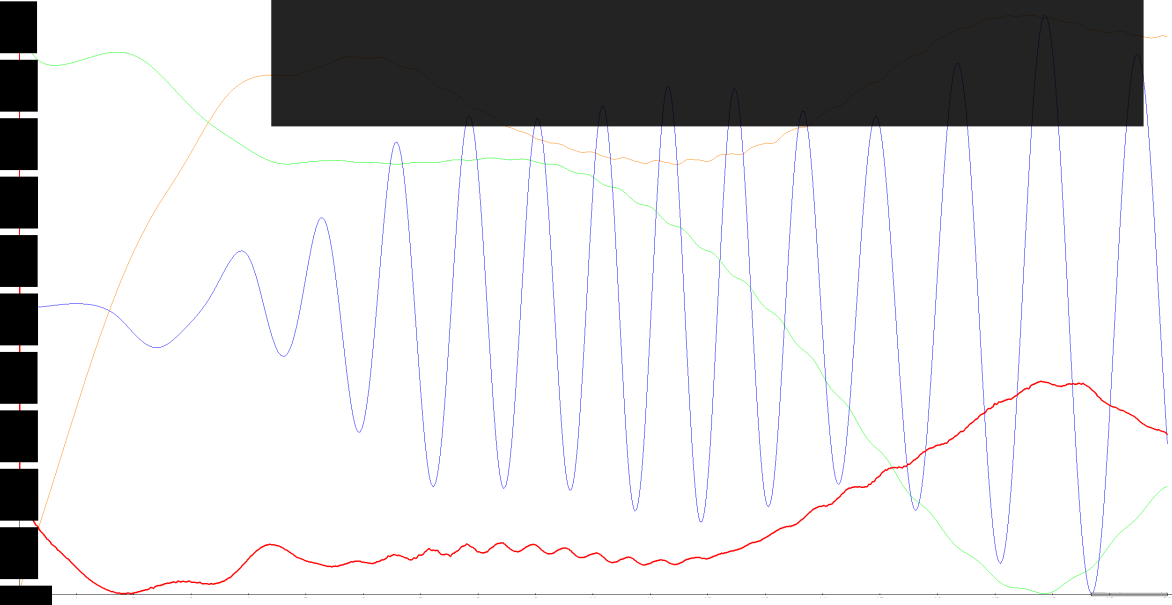
\includegraphics[height=5.5cm,width=0.55\textwidth]{q13.pdf}
    	\caption{Normalised goals plot for Average Static Pressure (red), Average
Velocity(X) (green), Average Velocity(Y) (blue) and Average Fluid Temperature
(orange) with physical time}
\label{fig:q13}
\end{figure}
Furthermore, the drag force acting on the uranium equilateral prism was
determined via use of surface parameters and shown to be $0.023~N$. This value
was then substituted into the following equation,
\begin{equation}
    C_{D}~=~\frac{F_{D}}{\frac{1}{2}\rho U^{2}DL}
\label{eq:dragcoef}
\end{equation}
in which $F_{D}$ is the drag force which has been determined, $U$ is the
velocity of the fluid, $D$ is the effective diameter of the uranium
equilateral prism (0.04m), $L$ is the length of the uranium equilateral prism
and $\rho$ is the fluid density of $CO_{2}$ ($29.25kgm^{-3}$). From
Equation \vref{eq:dragcoef}, the drag coefficient, $C_{D}$ was found to be
approximately 1.5, which is consistent with reference values for other
triangular prisms [4]. This means that the simulation may
be trusted in its calculated value of drag force, $F_{D}$. 
Again, by using the surface parameters feature, the heat removal rate from the
equilateral prism is found to be approximately 1.0kW.

% Q14


\begin{figure}
\centering
\begin{subfigure}{.49\textwidth}
  \centering
  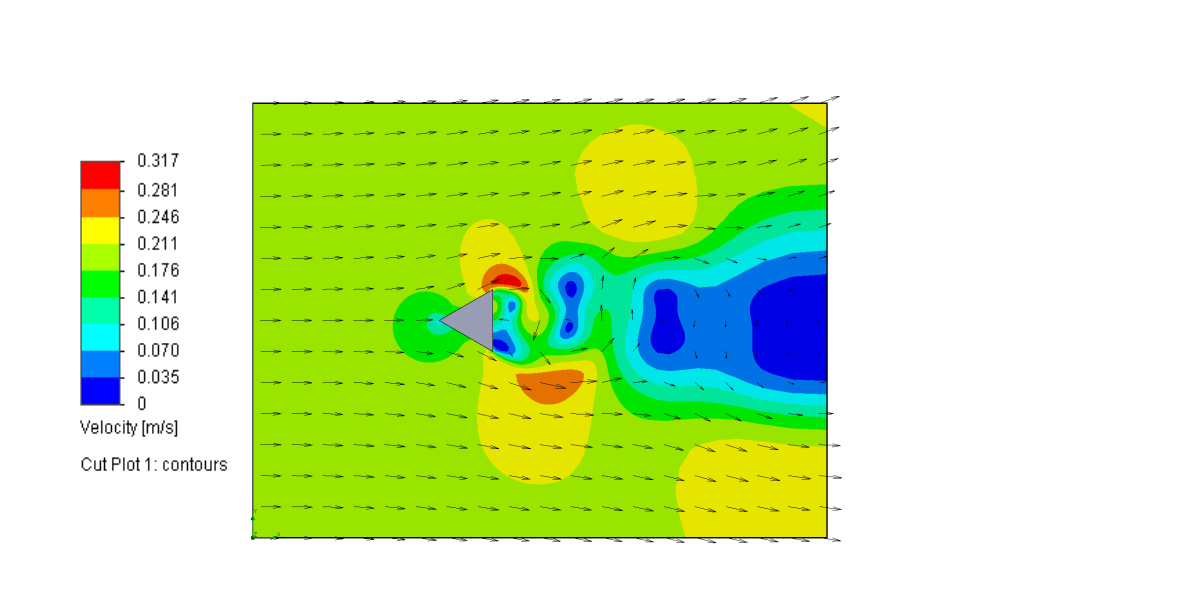
\includegraphics[width=1.7\linewidth]{q14.pdf}
  \caption{Cut plot showing contours of magnitude of fluid velocity and
vectors over two-dimensional domain}
\label{fig:q14}
\end{subfigure}
\begin{subfigure}{.49\textwidth}
  \centering
  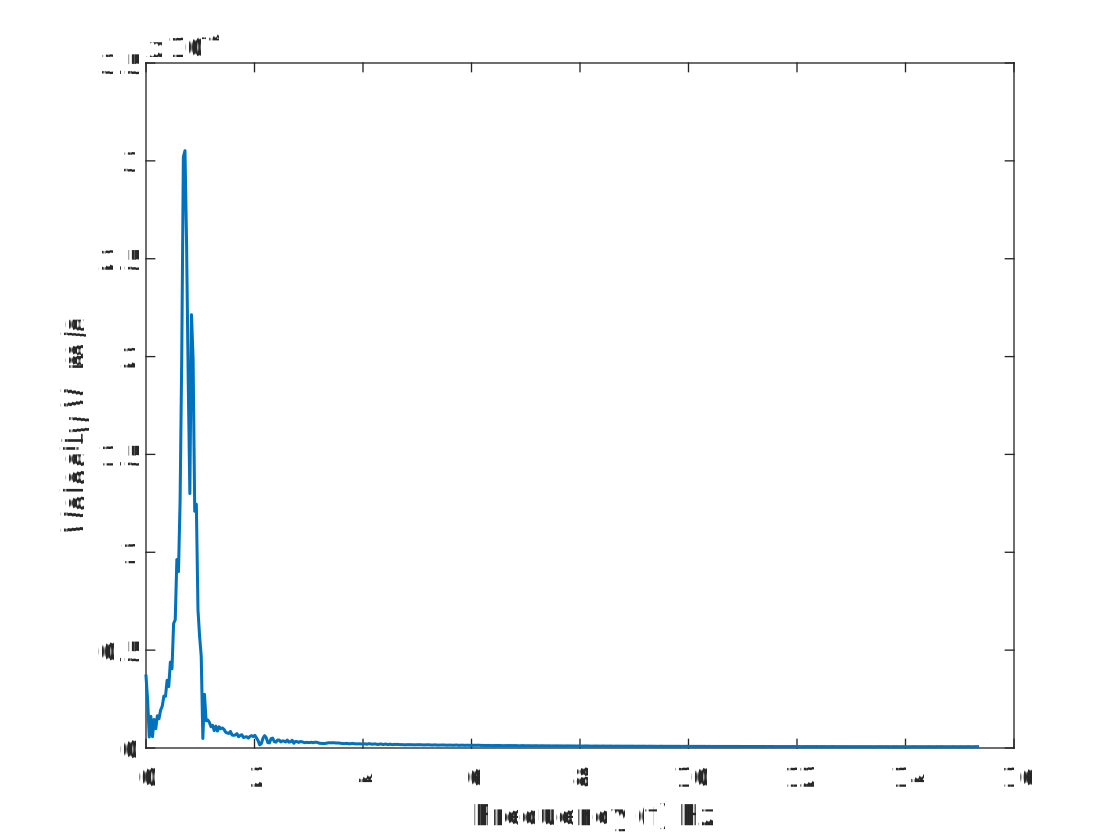
\includegraphics[width=\linewidth]{q17.pdf}
  \caption{Fast Fourier Transform (FFT) of Velocity (Y)}
  \label{fig:q17}
\end{subfigure}
\caption{Model II - "Coolant Flow"}
\end{figure}

As the Uranium equilateral prism is not streamlined, as the flow passes by it,
it causes an oscillating flow to occur (as can be seen by the Velocity (Y) in
Figure 5 on the previous page), this is referred to as 'Vortex Shedding' [5].
To determine the period of vortex shedding, a fast Fourier transform (FFT) was
performed in MATLAB\textregistered~on the Velocity (Y), as can be seen in
Figure 6(b).


The peak value occurs at a frequency of $0.7~Hz$, thus meaning that the period
of vortex shedding is $\frac{1}{0.7} = 1.4~s$.

To verify the obtained vortex shedding period, the Strouhal number may be used.
This is a dimensionless number which is a function of both the vortex shedding
frequency, $f$, and the Reynolds number, $Re$.
\begin{equation}
    S = 0.198(q-\frac{19.7}{Re}) = \frac{fD}{U}
    \label{eq:s}
\end{equation}
Through use of the above relationship, the theoretical and experimental
value of the Strouhal number may be compared. Calculating the Reynolds number
and substituting its value into Equation \ref{eq:s} yields a value of 0.20 for
the Strouhal number - this is validated by [4]. Now, calculating
the Strouhal number through use of the experimentally obtained vortex shedding
frequency gives a value of 0.14, which is $30\%$ smaller than the theoretical
value. If more accurate results were to be obtained from this simulation, using
a better - finer - mesh may be considered, or a more powerful computer which is
able to run the simulation with a smaller time step and therefore perform
more iterations within the 20~s time period. 

\section{References}
\begin{itemize}
\item [1] - $http://www.vttresearch.com/Documents/VTT_CFD_General.pdf$
\item [2] -
$https://www.team-consulting.com/insights/$\%$error-cfd-does-not-compute/$
\item [3] - Solidworks Flow Simulation: Instructor guide, p5.
\item [4] - Comparison of flow characteristics around an equilateral triangular
cylinder via PIV and Large Eddy Simulation methods
\item [5] - Sunden, B., 2011. Vortex shedding. Thermopedia.
\item [6] - $https://www.engineeringtoolbox.com/moody-diagram-d_618.html$
\end{itemize}









































\end{document}
